\section{Background and Previous Work}
\label{sec:mainsub_intro}

\gls{vqa} models are neural networks that answer natural language questions about an image by interpreting the question and the image provided~\cite{antol2015vqa,goyal2017making,hudson2019gqa,tan2019lxmert}. Specifying questions using natural language gives \gls{vqa} models great appeal, as the set of possible questions one can ask is enormous and does not need to be identical to the set of questions used to train the models. Due to these advantages, \gls{vqa} models for medical applications have also been proposed~\cite{gong2021cross,ImageCLEFVQA_Med2018,liao2020aiml,liu2019effective,vu2020question,zhan2020medical}, whereby allowing clinicians to probe the model with subtle differentiating questions and contributing to build trust in predictions.

To date, much of the work in \gls{medvqa} has focused on building more effective model architectures~\cite{gong2021cross,liao2020aiml,vu2020question} or overcoming limitations in \gls{medvqa} datasets~\cite{Nguyen19,liao2020aiml,sarrouti2020nlm,zhan2020medical}. Yet a critical component of \gls{vqa} is the notion of {\it consistency} in the answers produced by a model. Here, consistency refers to a model's capacity to produce answers that are not self-contradictory. For instance, the task of staging \gls{dme} from color fundus photograph illustrated in Fig.~\ref{fig:motivation} involves identifying {\it perception} elements in the image (\eg,~``are there hard exudates visible near the macula?'') to infer a disease stage, which can be expressed as a {\it reasoning} question (\eg,~``what is the stage of disease?''). Ultimately, for any \gls{vqa} model to be trustworthy, it should be able to answer these without contradicting itself (\ie, answer that the image is healthy, but also identify hard exudates in the periphery of the eye).
\begin{figure}[t]
\begin{center}
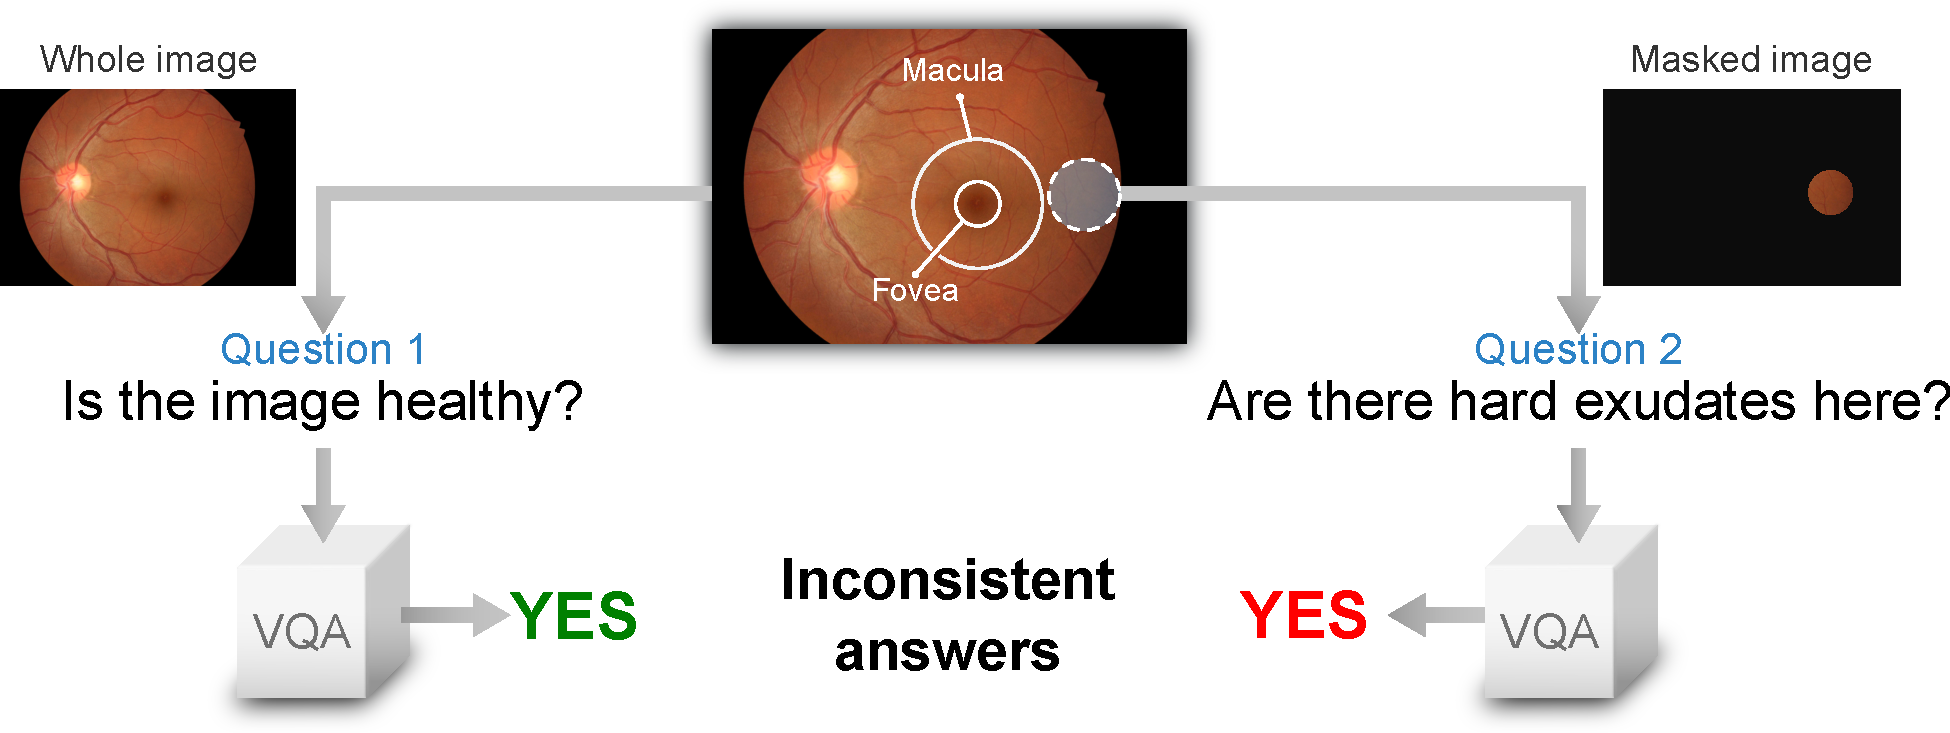
\includegraphics[width=0.75\textwidth]{Figures/Part2_Consist/01_mainsub/motivation_alt.pdf}
\caption{VQA inconsistency in Diabetic Macular Edema staging from fundus photograph. While the VQA model correctly answers ``Is the image healthy?" (left), it incorrectly answers yes to ``Are there hard exudates here?" for a specified retinal region (right).}
\label{fig:motivation}
\end{center}
\end{figure}

\nocite{wang2021image}

Consistency in \gls{vqa} has been been studied in the broader computer vision context~\cite{goel2021iq,gokhale2020vqa,ray2019sunny,ribeiro2019red,shah2019cycle}, where the relation between perception and reasoning questions is unconstrained. That is, the answers to perception questions do not necessarily imply any information with respect to the reasoning question and vice-versa. In these broad cases, some methods have modeled question implications \cite{ray2019sunny,ribeiro2019red} or rephrased questions~\cite{shah2019cycle} by generating tailored question-answer pairs (\eg,~consistent data-augmentation). Alternatively,~\cite{gokhale2020vqa,teney2019incorporating,yuan2021perception} used relations between questions to impose constraints in the \gls{vqa}'s embedding space. To avoid needing to know the relation between questions,~\cite{selvaraju2020squinting} proposed to enforce consistency by making attention maps of reasoning and perception questions similar to one another. 
However, even though these approaches tackle unconstrained question relations, the ensuring of \gls{vqa} models' consistency remains limited and often reduces the overall performance~\cite{selvaraju2020squinting}.  

Instead, we propose a novel approach to enforce \gls{vqa} consistency that is focused on cases where answers to the perception questions have explicit implications on reasoning question answers and vice-versa (\eg, cancerous cells and severity of cancer found in H\&E staining, or presence of hard exudates and \gls{dme} staging). By focusing on this subset of question relations, our aim is to improve both the accuracy of our model and its consistency, without needing external data as in~\cite{ribeiro2019red,Nguyen19,goel2021iq}. To do this, we allow questions to probe arbitrary image regions by masking irrelevant parts of the image and passing the masked image to the \gls{vqa} model (see Fig.~\ref{fig:motivation}). To then enforce consistency, we propose a new loss function that penalizes incorrect perceptual predictions when reasoning ones are correct for a given image. To validate the impact of our approach, we test it in the context of \gls{dme} staging and show that it outperforms state-of-the-art methods for consistency, without compromising overall performance accuracy. 